\documentclass[a4paper,12pt]{article} % тип документа

% Поля страниц
\usepackage[left=2.5cm,right=2.5cm,
    top=2cm,bottom=2cm,bindingoffset=0cm]{geometry}
    
%Пакет дял таблиц   
\usepackage{multirow} 
    
%Отступ после заголовка    
\usepackage{indentfirst}


% Рисунки
\usepackage{floatrow,graphicx,calc}
\usepackage{wrapfig}

%%% Работа с картинками
\usepackage{graphicx}  % Для вставки рисунков
\graphicspath{{images/}{images2/}}  % папки с картинками
\setlength\fboxsep{3pt} % Отступ рамки \fbox{} от рисунка
\setlength\fboxrule{1pt} % Толщина линий рамки \fbox{}
\usepackage{wrapfig} % Обтекание рисунков и таблиц текстом

% Создаёем новый разделитель
\DeclareFloatSeparators{mysep}{\hspace{1cm}}

% Ссылки?
\usepackage{hyperref}
\usepackage[rgb]{xcolor}
\hypersetup{				% Гиперссылки
    colorlinks=true,       	% false: ссылки в рамках
	urlcolor=blue          % на URL
}


%  Русский язык
\usepackage[T2A]{fontenc}			% кодировка
\usepackage[utf8]{inputenc}			% кодировка исходного текста
\usepackage[english,russian]{babel}	% локализация и переносы

% Математика
\usepackage{amsmath,amsfonts,amssymb,amsthm,mathtools}

%%% Дополнительная работа с математикой
\usepackage{amsmath,amsfonts,amssymb,amsthm,mathtools} % AMS
\usepackage{icomma} % "Умная" запятая: $0,2$ $-$- число, $0, 2$ $-$- перечисление


% Что-то 
\usepackage{wasysym}


\begin{document}
\begin{center}
	\footnotesize{МОСКОВСКИЙ ФИЗИКО-ТЕХНИЧЕСКИЙ ИНСТИТУТ\\(НАЦИОНАЛЬНЫЙ 			ИССЛЕДОВАТЕЛЬСКИЙ УНИВЕРСИТЕТ)}\\
	\footnotesize{ФИЗТЕХ-ШКОЛА РАДИОТЕХНИКИ И КОМПЬЮТЕРНЫХ ТЕХНОЛОГИЙ\\}
	\hfill \break
	\hfill \break
	\hfill \break
	\hfill \break
	\hfill \break
	\hfill \break
\end{center}

\begin{center}   
    \hfill \break
	\hfill \break
	\hfill \break
	\hfill \break
	\hfill \break
	\hfill \break
	\hfill \break
	\hfill \break
	\hfill \break
	\hfill \break
	\hfill \break
	\large{Лабораторная работа № 4.1.1\\\large{\textbf{Изучение центрированных оптических систем}}}\\
	\hfill \break
        \hfill \break
	\hfill \break
	\hfill \break
	\hfill \break
	\hfill \break
	\hfill \break
	\hfill \break
	\hfill \break
	\hfill \break
	\hfill \break
	\begin{flushright}
		Климова Екатерина\\
		Группа Б01-108
	\end{flushright}
	\hfill \break
\end{center}
\hfill \break
\hfill \break
\begin{center}
	Долгопрудный, 2023 г.
\end{center}
\thispagestyle{empty}

\newpage
\hfill \break
\textbf{Цель работы:} изучить методы определения фокусных расстояний линз и сложных оптических систем; определить характеристики оптической системы, составленной из тонких линз; изучить недостатки реальных линз $-$ сферическую и хроматическую аберрации.
\hfill \break
\hfill \break
\textbf{В работе используются:} оптическая скамья с набором рейтеров; положительные и отрицательные линзы; экран; осветитель с ирисовой диафрагмой; зрительная труба; светофильтры; кольцевые диафрагмы; линейка.

\section{Аннотация}
\hfill \break В первой части работы предлагается определить фокусные расстояния тонких собирающих и рассеивающих линз, рассчитать их оптическую силу, а также определить фокусное расстояние и положения главных и фокальных плоскостей оптической системы из двух тонких линз.

\hfill \break Во второй части проводится исследование аберраций плосковыпуклой линзы: набор кольцевых диафрагм позволяет исследовать продольную сферическую аберрацию (зависимость фокусного расстояния от радиуса кольцевого пучка, падающего на линзу), а набор светофильтров $-$ хроматическую аберрацию (зависимость фокусного расстояния от длины волны).

\section{Теоретические сведения}

\subsection*{А. Определение фокусных расстояний тонких линз и характеристик сложной оптической системы}

\hfill \break Оптические приборы, предназначенные для формирования изображений, в большинстве случаев представляют собой так называемые \textit{центрированные оптические системы} $-$ однородные преломляющие или отражающие среды, отделенные одна от другой сферическими поверхностями, центры кривизны которых лежат на одной прямой, называемой \textit{главной оптической осью}.

\hfill \break Получаемые с помощью оптических систем действительные или мнимые изображения образуются световыми пучками, которые называются \textit{гомоцентрическими}, если, выйдя из одной точки и пройдя оптическую систему, пучки или их продолжения снова сходятся в одной точке.

\hfill \break \textit{Идеальной оптической системой} называют систему, в которой имеет место гомоцентричность пучков и изображение подобно предмету. Идеальная оптическая система может быть реализована с достаточным приближением в виде центрированной оптической системы, если при формировании изображения ограничиться \textit{параксиальными пучками}, то есть пучками, идущими вблизи оси симметрии.

\begin{center}
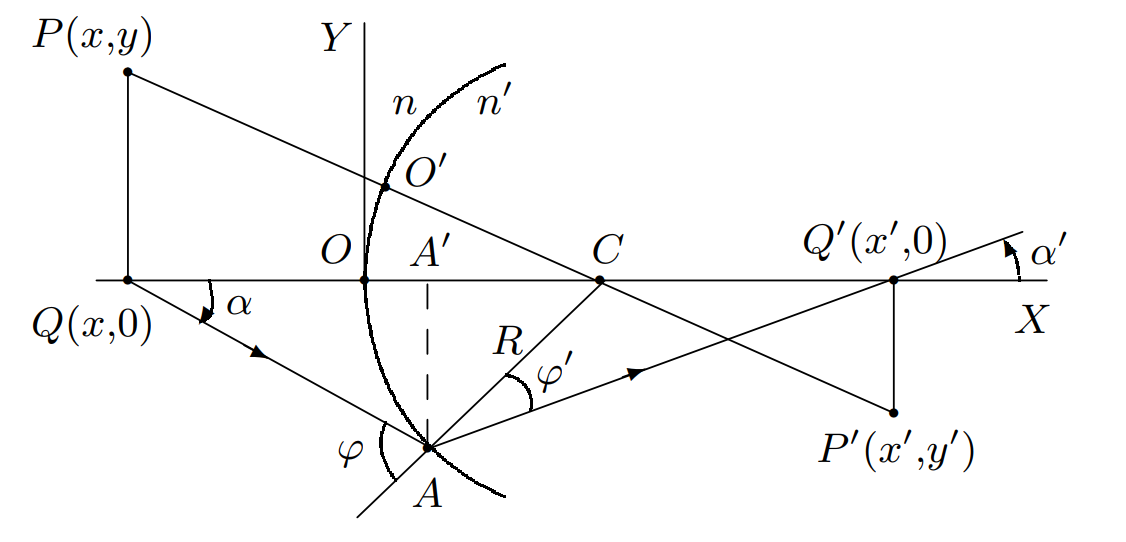
\includegraphics[width=0.75\textwidth]{4.1.1_1.png}\\
\textbf{Рис. 1.} Элементарная оптическая ячейка \\
\end{center}

\hfill \break Используя закон преломления, получим для элементарной оптической ячейки, изображённой на рис. 1, в параксиальном приближении:

\begin{equation}\label{опт-ячейка}
	-\frac{n}{x}+\frac{n'}{x'} = \frac{n'-n}{R},
\end{equation}

\begin{equation}
	x \alpha = x' \alpha'.
\end{equation}

\hfill \break Для прямой $ P P' $, рассмотренной как оптическая ось, 

\begin{equation}\label{PP}
	\frac{y'}{y} = \frac{x' - R}{x - R}.
\end{equation}

\hfill \break Проведя замену переменных, получим систему уравнений

\begin{equation}\label{grid}
	\frac{x' - F'}{H' - F'}= \frac{H-F}{x- F} = \frac{y'}{y} = \frac{n \alpha}{n' \alpha'},
\end{equation}

\begin{equation}\label{grid1}
	(x-H)\alpha= (x' - H')\alpha'.
\end{equation}

\hfill \break Из этих уравнений получим

\begin{equation}\label{Ф}
	\frac{n}{f} = -\frac{n'}{f'} \equiv \Phi,
\end{equation}

\hfill \break где

\begin{equation}\label{focus-len}
	f\equiv H - F, \;\;\; f'\equiv H' - F'.
\end{equation}

\hfill \break $ f $ и $ f' $ $-$ главные фокусные расстояния системы.

\subsubsection*{I. Определение фокусного расстояния тонкой собирающей линзы и сложных оптических систем по методу Аббе}
\hfill \break Измерение фокусного расстояния по методу Аббе основано на определении поперечного увеличения для нескольких (не менее двух) различных положений предмета, находящегося на оптической оси исследуемой оптической системы. На рис. 2 представлена соответствующая схема эксперимента.

\begin{center}
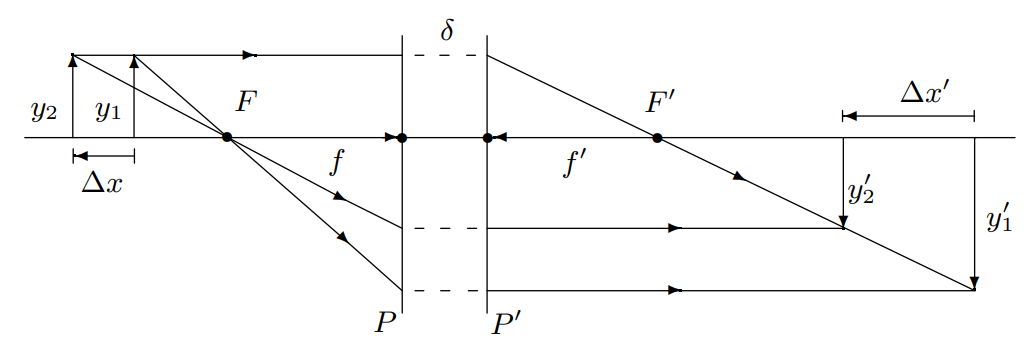
\includegraphics[width=0.75\textwidth]{4.1.1_2.png}\\
\textbf{Рис. 2.} Измерение фокусного расстояния оптической системы по методу Аббе \\
\end{center}

\hfill \break С учетом определения (7) и формул (4), (6), фокусное расстояние системы можно выразить через положения предмета и соответствующие увеличения следующим образом:

\begin{equation}
    f = \frac{\Delta x}{\Delta (y/y')} = - \frac{\Delta x'}{\Delta (y'/y)}.
\end{equation}

\hfill \break Здесь $\Delta x = x_2 - x_1$ $-$ смещение предмета, $\Delta x' = x_2' - x_1'$ $-$ соответствующее ему перемещение изображения, $\Delta (y'/y) = y_2/y_2' - y_1/y_1'$ $-$ приращение поперечного увеличения, а $\Delta (y/y')$ $-$ приращение величины, обратной поперечному увеличению. Для повышения точности измерений следует выбирать такие смещения $\Delta x$, чтобы увеличения заметно отличались друг от друга. С целью уменьшения случайной ошибки, возникающей при фокусировке изображения, измерения следует проводить несколько раз, усредняя полученные данные.

\hfill \break Основное достоинство метода Аббе состоит в том, что фокусное расстояние сложной системы или линзы, как это видно из рисунка, может быть получено при неизвестном расстоянии $\delta$ между главными плоскостями $P$ и $P'$.

\subsubsection*{II. Определение фокусного расстояния собирающих линз и сложных оптических систем по методу Бесселя}

\hfill \break Схема метода Бесселя для случая, когда $n = n'$ и $f' = -f$, представлена на рис. 3. 

\hfill \break Пусть начала координатных систем помещены в главные точки. В новых переменных $s \equiv x - H$, $s' \equiv x' - H'$. При сохранении прежних обозначений для поперечных координат уравнения (4) принимают вид

\begin{equation}
    \frac{s' + f'}{f'} = \frac{f}{s + f} = \frac{y'}{y} = \frac{n}{n'} \frac{\alpha}{\alpha'}.
\end{equation}

\hfill \break Первое уравнение этой системы можно представить в виде, подобном формуле тонкой линзы

\begin{equation} \label{23}
    \frac{f}{s} + \frac{f'}{s'} = -1
\end{equation}

\hfill \break с разными фокусными расстояниями, связанными соотношением (6). Пусть среда по обе стороны оптической системы одна и та же. В диоптрической системе $n = n'$, и по формуле (6) $f = -f'$. При этом угловое увеличение есть величина, обратная поперечному увеличению, и узловые точки системы совпадают с главными точками. Вместо (10) имеем

\begin{equation} \label{24}
    -\frac{1}{s} + \frac{1}{s} = \frac{1}{f}.
\end{equation}

\begin{center}
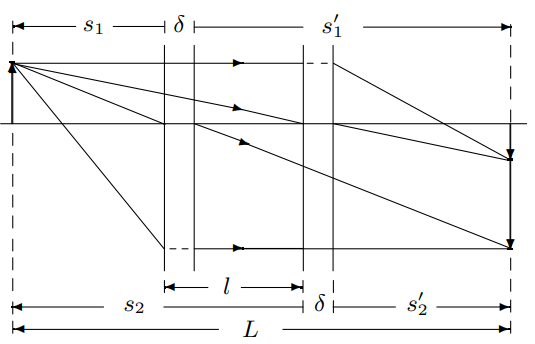
\includegraphics[width=0.65\textwidth]{4.1.1_3.png}\\
\textbf{Рис. 3.} Измерение фокусного расстояния оптической системы по методу Бесселя \\
\end{center}

\hfill \break Метод Бесселя основан на том, что при заданном расстоянии $L$ между предметом и экраном уравнение (11) представляет собой квадратное уравнение относительно расстояния $s$ от главной плоскости пространства предметов до предмета ($s < 0$):

\begin{equation}
    -\frac{1}{s} + \frac{1}{L - \delta + s} = \frac{1}{f},
\end{equation}

\hfill \break имеющее при условии $L > 4f + \delta$ решения $s_1$ и $s_2$, показанные на рис. 3, где $\delta$ $-$ расстояние между главными плоскостями системы (линзы).\\

\hfill \break С учетом симметрии и направлений измерения расстояний, положения предметов определяются соотношениями $s_2' = -s_1$ и $s_1' = -s_2$. Для расстояния $L$ между предметом и экраном и расстояния $l$ между двумя положениями системы (линзы) получаем: $L - \delta = s_1' - s_1$, $l = -s_2 + s_1 = s_1 + s_1'$. Отсюда следует, что

\begin{equation}\label{ss}
    s_1 = - \frac{1}{2}(L - \delta - l), \qquad s_1' = \frac{1}{2}(L - \delta + l).
\end{equation}

\hfill \break Подставляя (13) в (10), находим выражение

\begin{equation}\label{4}
    f = \frac{(L - \delta)^2 - l^2}{4(L - \delta)}.
\end{equation}

\hfill \break Если выполняется условие $|\delta| \ll L$, то с относительной погрешностью

\begin{equation*}
    \varepsilon_f = \frac{L^2 + l^2}{L^2 - l^2} \frac{|\delta|}{L}
\end{equation*}

\hfill \break формула (14) может быть представлена в более простом виде

\begin{equation}
    f = \frac{L^2 - l^2}{4L}.
\end{equation}

\hfill \break Для определения фокусного расстояния $f$ достаточно, таким образом, измерить расстояние $L$ между предметом и экраном и расстояние $l$ между двумя положениями системы, при которых на экране видны чёткие изображения. Допускаемая при этом относительная погрешность результата измерений (без учёта случайных ошибок) даже для толстых линз и некоторых сложных оптических систем может быть мала.

\hfill \break В данной работе будем выполнять измерения по \textbf{методу Бесселя}.

\subsubsection*{III. Определение фокусного расстояния тонкой собирающей линзы}

\hfill \break Если собирающую линзу можно считать тонкой, т. е. принять, что главные плоскости линзы совпадают, то её фокусное расстояние может быть измерено, например, следующими способами (в дополнение к изложенным выше).

\hfill \break \textbf{Способ 1.} Воспользуемся формулой тонкой линзы:

\begin{equation}\label{thin}
    -\frac{1}{a} + \frac{1}{a'} = \frac{1}{f}.
\end{equation}

\hfill \break Здесь $a$ и $a'$ $-$ расстояния до предмета и его изображения от плоскости линзы, причем $a < 0$, $a' > 0$, если предмет находится слева, а его изображение $-$ справа от линзы; фокусное расстояние $f > 0$.

\hfill \break Для измерения фокусного расстояния достаточно провести измерения по стандартной схеме <<предмет — линза — экран>> при произвольном расстоянии между предметом и экраном с различными значениями $a$ при увеличенном и при уменьшенном изображении. Относительная погрешность определения фокусного расстояния линзы по этому методу порядка $d/f$, где $d$ — толщина линзы. Сравнение среднеквадратичного отклонения измеренных значений $f$ от среднего $d$ позволит сделать вывод о том, нужны ли многократные измерения.

\hfill \break \textbf{Способ 2.} Фокусное расстояние тонкой собирающей линзы можно определить с помощью зрительной трубы, настроенной на бесконечность, то есть на параллельный пучок лучей. Разместив между предметом и зрительной трубой положительную линзу и перемещая её вдоль оси системы, можно найти резкое изображение предмета в окуляре зрительной трубы. При этом расстояние от середины линзы до предмета равно фокусному расстоянию тонкой линзы. Для толстой линзы зрительная труба позволяет определить только положение главного фокуса. 

\subsubsection*{IV. Определение фокусного расстояния тонкой рассеивающей линзы}
\hfill \break \textbf{Способ 1.} Определение фокусного расстояния рассеивающей линзы затруднено тем, что изображение предмета получается мнимым (при действительном источнике) и поэтому не может быть получено на экране. Эту трудность легко обойти с помощью вспомогательной собирающей линзы.

\begin{center}
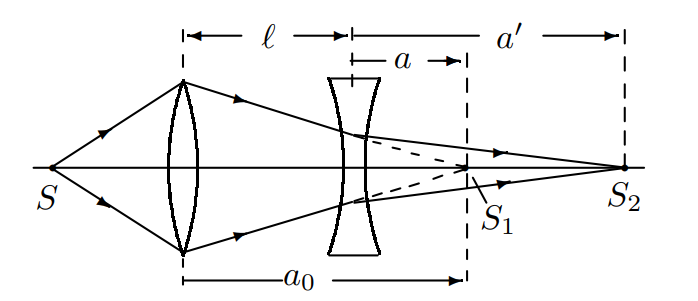
\includegraphics[width=0.75\textwidth]{4.1.1_4.png}\\
\textbf{Рис. 4.} Измерение фокусного расстояния рассеивающей линзы \\
\end{center}

\hfill \break Сначала с помощью собирающей линзы получают на экране действительное изображение предмета $S$ (точка $S_1$ на рис. 4). Затем на пути лучей, выходящих из собирающей линзы, располагают исследуемую рассеивающую линзу и, отодвигая экран, получают чёткое изображение предмета на экране, образованное двумя линзами. Точка $S_1$ пересечения сходящихся лучей играет по отношению к рассеивающей линзе роль мнимого источника. Изображение источника переместится теперь в точку $S_2$.

\hfill \break Определив расстояния $a = a_0 - l > 0$ и $a^\prime > 0$, рассчитывают фокусное расстояние рассеивающей линзы по формуле (16), которое, естественно, должно получиться отрицательным.

\hfill \break \textbf{Способ 2.} Если расстояние $a$ на рис. 4 совпадает с модулем фокусного расстояния рассеивающей линзы, то изображение $S_2$ перемещается в бесконечность, то есть лучи выходят из линзы параллельным пучком.

\hfill \break Параллельность пучка можно установить с помощью зрительной трубы, настроенной на бесконечность. Зная расстояние от первой линзы до точки $S_1$ и расстояние между линзами, нетрудно определить фокусное расстояние тонкой рассеивающей линзы. Для толстой отрицательной линзы этот метод позволяет определить только положение главного фокуса.

\subsubsection*{V. Определение положения главных и фокальных плоскостей сложной оптической системы}

\hfill \break Для нахождения главных плоскостей системы недостаточно знать фокусное расстояние, нужно определить ещё положения главных фокусов. Это можно сделать при помощи зрительной трубы, настроенной на бесконечность. Отложив от главных фокусов отрезки, равные фокусному расстоянию, можно найти положения главных плоскостей системы. При этом необходимо учитывать возможность различного взаимного расположения кардинальных точек (плоскостей) сложной системы.

\hfill \break Все характеристики оптической системы, состоящей из двух тонких линз, можно рассчитать, если известны фокусные расстояния $f_1$, $f_2$ каждой линзы и оптический интервал $\Delta$ или расстояние между центрами линз $l_{12}$.

\subsection*{Б. Аберрации реальных оптических систем}
	
\subsubsection*{I. Сферическая аберрация}
\hfill \break Сферическая аберрация возникает при преломлении широких (не параксиальных) пучков света на сферических поверхностях линз. Рис. 5 поясняет возникновение сферической аберрации.

\begin{center}
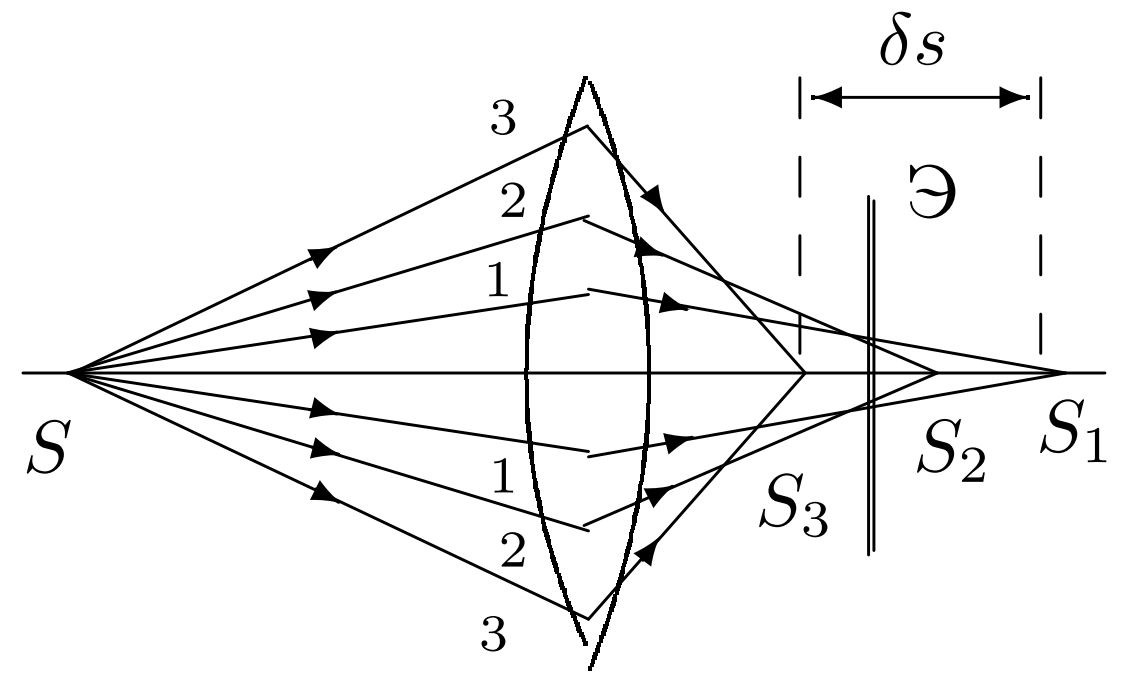
\includegraphics[width=0.5\textwidth]{4.1.1_5.png}\\
\textbf{Рис. 5.} Сферическая аберрация \\
\end{center}

\hfill \break Приведем приближенные формулы для плосковыпуклой (или плосковогнутой) линзы, на плоскую поверхность которой падает широкий параллельный пучок света.

\begin{center}
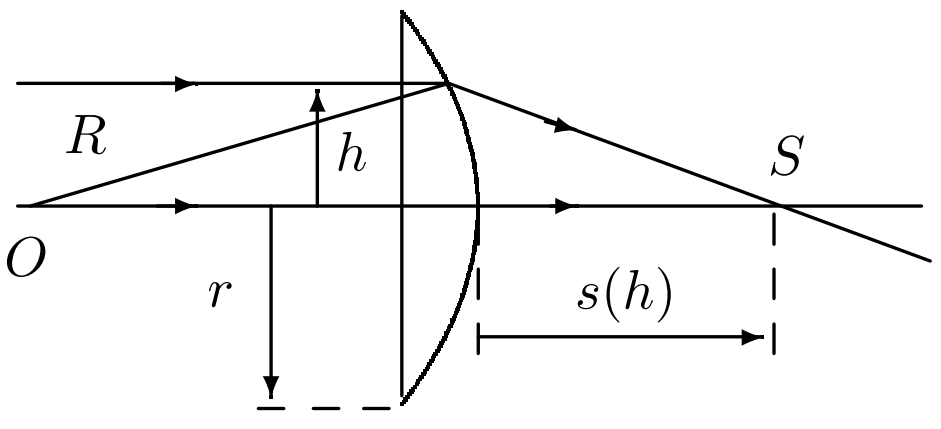
\includegraphics[width=0.5\textwidth]{4.1.1_7.png}\\
\textbf{Рис. 6.} Сферическая аберрация плосковыпуклой линзы \\
\end{center}

\hfill \break Для лучей, проходящих на расстоянии $h$ от центра линзы, расстояние $s$ выражается соотношением:
	
 \begin{equation}
s = \frac{R}{n - 1}\left(1 - \frac{1}{2} \frac{n^2 h^2}{R^2}\right).
\end{equation}

\hfill \break Характеристической кривой сферической аберрации называют зависимость 

\begin{equation}
\delta s(h) = s(h) - s(0) = -\frac{1}{2}\frac{n^2 h^2}{(n - 1)R} = -\frac{1}{2}\left(\frac{n}{n - 1}\right)^2 \left(\frac{h}{f}\right)^2 f.
\label{eq:8}
\end{equation}

\hfill \break При $h = r$ — радиус линзы, формула определяет продольную сферическую аберрацию линзы.

\subsubsection*{II. Хроматическая аберрация}
\hfill \break Хроматическая аберрация (зависимость фокусного расстояния линзы от длины волны) возникает вследствие дисперсии показателя преломления стёкол, т. е. из-за того, что показатель преломления $n = n(\lambda)$. Возникновение хроматической аберрации поясняет рис. 7.

\begin{center}
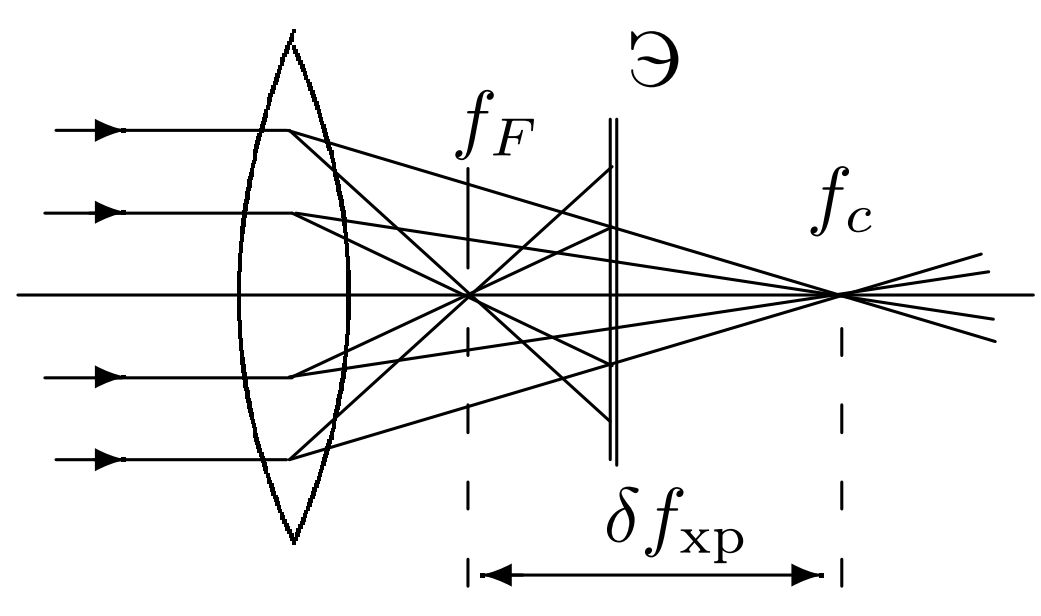
\includegraphics[width=0.45\textwidth]{4.1.1_6.png}\\
\textbf{Рис. 7.} Хроматическая аберрация \\
\end{center}

\hfill \break Хроматическую аберрацию принято характеризовать разностью фокусных расстояний для двух характерных спектральных линий водорода, расположенных в крайних частях видимой области спектра: $\lambda_F$ = 430 нм (голубая линия $F$ водорода), $\lambda_C$ = 630 нм (красная линия $C$ водорода):

\begin{equation}
	\delta f_{\text{хр}} = f_F - f_C.
    \label{eq:9}
\end{equation}

\hfill \break Для характеристики дисперсионных свойств стёкол часто пользуются так называемым коэффициентом дисперсии, или числом Аббе:
	
\begin{equation}
\nu = \frac{n_D - 1}{n_F - n_C},
\end{equation}

\hfill \break где $n_D$ $-$ показатель преломления для оранжевой линии $D$ натрия $\lambda_D$ = 580 нм. Тогда:

\begin{equation}
\delta f_{\text{хр}} = -\frac{1}{\nu} f_D.
\label{eq:11}
\end{equation}

\section{Экспериментальная установка}
\hfill \break Оптическая скамья с осветителем, транспарант, набор линз, экран и зрительная труба позволяют определить параметры оптических систем всеми описанными способами. Все оптические элементы устанавливаются на скамье при помощи рейтеров.

\hfill \break Важную роль играет правильная центрировка элементов системы. Проходя через плохо отцентрированную систему, лучи света могут отклониться и пройти мимо экрана или глаза наблюдателя. Центрировать линзы следует как по высоте, так и в поперечном направлении, для чего линзы установлены на поперечных салазках.

\section{Ход работы}
\subsection*{А. Определение фокусных расстояний тонких линз и характеристик сложной оптической системы}
\hfill \break Из имеющегося комплекта линз отберем собирающие, затем соберем и отцентрируем установку и собирающую линзу. Отодвинем экран от осветителя и разместим в промежутке рейтер с собирающей линзой №1. Передвигая линзу и экран вдоль скамьи, добьемся четкого изображения края ирисовой диафрагмы осветителя на экране. Закрепим рейтеры. Смещая линзу с помощью поперечных салазок и по высоте, приведем центр изображения к центру экрана. Таким образом отцентрируем все положительные линзы, добавляя их последовательно к системе. Оптические оси линз устанавливаем параллельно ребру оптической скамьи.

\hfill \break Для центрировки рассеивающих линз можем воспользоваться уже отцентрированной положительной линзой, расположив ее впереди отрицательной.

\subsubsection*{I. Определение фокусных расстояний тонких линз при помощи экрана}
\hfill \break Воспользуемся \textbf{методом Аббе} для определения фокусного расстояния тонкой собирающей линзы №1. Закрепим линзу между осветителем и экраном. Перемещая осветитель вдоль скамьи, получим на экране резкое изображение предмета (стрелки размером 2 см) при двух различных положениях осветителя и соответственно экрана. 

\hfill \break Зафиксируем перемещение предмета $\Delta x = (3.5 \pm 0.2)$ см, перемещение изображения $\Delta x^\prime = -32.5$ см, размер изображения до перемещения $-$ $y_{1}^\prime = 4.15$ см и после $-$ $y_{2}^\prime = 85$ см, размер предмета $y = 1.8$ см, $y_{1} = 52.5$ см и $y_{2} = 10.6$ см. Тогда согласно формулам (8):

$$
\Delta \left( \frac{y^\prime}{y} \right) = \frac{y_{2}^\prime}{y_{2}} - \frac {y_{1}^\prime} {y_{1}} = 3.58 \pm 0.4; \text{ } \Delta \left( \frac{y}{y^\prime} \right) = \frac{y_{2}}{y_{2}^\prime} - \frac {y_{1}} {y_{1}^\prime} = 0.26 \pm 0.04.
$$

\begin{equation}\label{ linkname }
\Rightarrow f = \frac {\Delta x} {\Delta \left( y / y^\prime \right)} = (13 \pm 3) \text{ см}; \text{ } f = - \frac {\Delta x^\prime} {\Delta \left( y^\prime / y \right)} = (9 \pm 1) \text{ см}.
\end{equation}
 
\hfill \break Видно, что полученные значения фокусного расстояния совпадают в пределах погрешности.

\hfill \break Теперь измерим фокусное расстояние той же линзы №1 при помощи \textbf{метода Бесселя}. Установим линзу между осветителем и экраном. Расположим экран на расстоянии $L > 4f$ от предмета (рис. 3). Перемещая линзу вдоль скамьи, получим увеличенное и уменьшенное изображения предмета на экране. 

\begin{wrapfigure}{l}{0.35\textwidth}
\begin{center}
    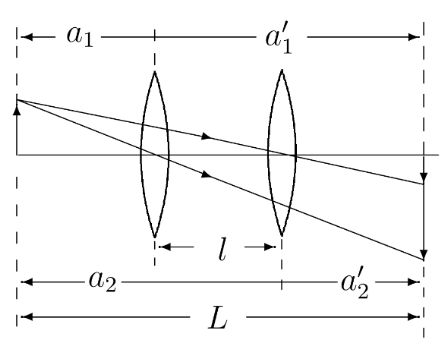
\includegraphics[width=1\textwidth]{4.1.1_8.png}
    \textbf{Рис. 8.} К определению фокусного расстояния тонкой собирающей линзы методом Бесселя
\end{center}
\end{wrapfigure}

\hfill \break Из соображений симметрии ясно, что $a_{1} = a_{2}^\prime$ и $a_{2} = a_{1}^\prime$ (рис. 8). Обозначая расстояние между предметом и экраном через $L$ и расстояние между двумя положениями линзы через $l$, получим: 

\begin{equation}\label{ linkname }
L = a_{1} + a_{2} = a_{1}^\prime + a_{2}^\prime; \text{ } l = a_{2} - a_{1} = a_{1}^\prime - a_{2}^\prime.
\end{equation}

\hfill \break Отсюда следует:

$$
a_{1} = \frac{L - l} {2}; \text{ } a_{1}^\prime = \frac {L + l} {2}.
$$

\hfill \break
\hfill \break Тогда, подставив это в формулу линзы, найдем фокусное расстояние:

\begin{equation}\label{ linkname }
f = \frac {L^2 - l^2} {4L}.
\end{equation}

\hfill \break С помощью линейки измерим расстояния от линзы до предмета и до изображения. При фиксированном расстоянии $L$ между осветителем и экраном, слегка перемещая линзу, повторим измерения несколько раз для разных значений $L$. Для каждого измерения будем фиксировать фокусное расстояние, а затем усредним результат. 

\begin{center}
\begin{tabular}{|c|c|c|c|c|c|}\hline
$ L $, см & $ a_{1} $, см & $ a_{1}^\prime $, см & $ l $, см & $ f $, см & $ \sigma_f $, см \\\hline
100.2 & 12.6 & 88.1 & 75.5 & 10.8 & 0.1 \\\hline
90.0 & 12.7 & 77.4 & 64.7 & 10.9 & 0.1 \\\hline
80.0 & 13.2 & 66.8 & 53.6 & 11.0 & 0.1 \\\hline
70.0 & 13.5 & 56.5 & 43.0 & 10.9 & 0.1 \\\hline
60.0 & 14.4 & 45.6 & 31.2 & 10.9 & 0.1 \\\hline
\end{tabular} \\
\hfill \break \textbf {Таблица 1.} Определение фокусного расстояния тонкой собирающей линзы методом Бесселя\\
\end{center}

\hfill \break Тогда, усредняя результат, получим $f_{\text{ср}} = 10.9$ см. Погрешность определения фокусного расстояния найдем как $\sigma_{f_{\text{ср}}} = \sqrt{ \sigma_{f}^2 + \sigma_{\text{ср}}^2} \approx 0.1$ см, где $\sigma_{\text{ср}} = \sqrt{ \frac{1} {5 \cdot 4} \sum\limits_{i = 1}^5 (f_{i} - f_{\text{ср}})^2 }$. Таким образом, $f_{\text{ср}} = (10.9 \pm 0.1)$ см.

\hfill \break Проведем те же расчеты, используя \textbf{формулу тонкой линзы} (16):

$$
- \frac{1}{a} + \frac{1} {a^\prime} = \frac{1}{f},
$$

\hfill \break где $a$ и $a^\prime$ $-$ расстояния до предмета и его изображения от плоскости линзы.
\hfill \break

\begin{center}
\begin{tabular}{|c|c|c|c|}\hline
$ a $, см & $ a^\prime $, см & $ f $, см & $ \sigma_f $, см \\\hline
12.6 & 89.6 & 11.0 & 0.1 \\\hline
12.7 & 78.5 & 10.9 & 0.1 \\\hline
13.2 & 68.0 & 11.1 & 0.1 \\\hline
13.5 & 57.7 & 10.9 & 0.1 \\\hline
14.4 & 47.8 & 11.1 & 0.1 \\\hline
\end{tabular} \\
\hfill \break \textbf {Таблица 2.} Определение фокусного расстояния тонкой собирающей линзы по формуле тонкой линзы\\
\end{center}

\hfill \break Отсюда, аналогично, получим: $f = (11.0 \pm 0.1)$ см.

\begin{wrapfigure}{r}{0.35\textwidth}
\begin{center}
    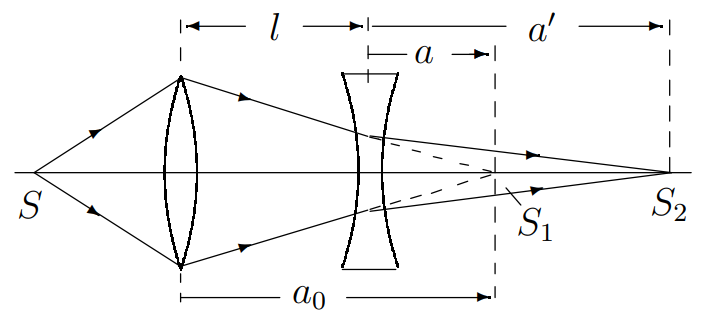
\includegraphics[width=1\textwidth]{4.1.1_9.png}
    \textbf{Рис. 9.} Измерение фокусного расстояния отрицательной линзы
\end{center}
\end{wrapfigure}

\hfill \break Для определения фокусного расстояния \textit{тонкой отрицательной линзы} сначала с помощью одной собирающей линзы №1 получим на экране увеличенное изображение предмета и измерим расстояние от центра линзы до экрана ($a_{0}$ на рис. 9). Затем между собирающей линзой и экраном разместим рассеивающую линзу и, отодвигая экран от линзы, найдем действительное изображение предмета, образованное системой линз.

\hfill \break Используем измеренные величины: $a^\prime$ $-$ расстояние от рассеивающей линзы до экрана и $l$ $-$ расстояние между линзами. Рассчитаем величину $a$ и определим фокусное расстояние рассеивающей линзы с помощью формулы тонкой линзы (16):

$$
l = (27.2 \pm 0.1) \text{ см}; \text{ } a^\prime = (64.2 \pm 0.1) \text{ см}; \text{ } a_{0} = (33.3 \pm 0.1) \text{ см};
$$

$$
a = a_{0} - l = (6.1 \pm 0.1) \text{ см}.
$$

$$
\Rightarrow f_{\text{расс}} = - \frac {a \cdot a^\prime} {a + a^\prime} = (-6.7 \pm 0.3) \text{ см}.
$$

\subsubsection*{II. Определение фокусных расстояний тонких линз с помощью зрительной трубы}
\hfill \break Для определения фокусных расстояний линз с помощью зрительной трубы настроим трубу на бесконечность. Поставим \textit{собирающую линзу №1} на расстоянии от предмета, примерно равном фокусному расстоянию. На небольшом расстоянии от линзы закрепим трубу, настроенную на бесконечность, и отцентрируем ее по высоте. Передвигая линзу вдоль скамьи, получим в окуляре зрительной трубы четкое изображение предмета. При этом расстояние между предметом и серединой линзы равно фокусному расстоянию:

$$
f_{\text{1 №1}} = (11.6 \pm 0.1) \text{ см}.
$$

\hfill \break Повернем линзу другой стороной к источнику и повторим измерения фокусного расстояния:

$$
f_{\text{2 №1}} = (9.8 \pm 0.1) \text{ см}.
$$

\hfill \break $\Rightarrow$ линзу №1 можно считать тонкой с достаточно хорошей точностью, так как полученные значения близки. Аналогичным образом измерим фокусное расстояние \textit{собирающей линзы №2}:

$$
f_{\text{1 №2}} = (13.9 \pm 0.1) \text{ см};
$$

$$
f_{\text{2 №2}} = (13.9 \pm 0.1) \text{ см}.
$$

\hfill \break Следовательно, линзу №2 также можно считать тонкой. 

\hfill \break Для определения фокусного расстояния тонкой \textit{рассеивающей линзы} воспользуемся схемой, изображенной на рис. 9. Сначала получим на экране увеличенное изображение предмета при помощи короткофокусной положительной линзы. Измерим расстояние между линзой и экраном: $a_{0} = 31.7$ см. Закрепим сразу за экраном трубу, настроенную на бесконечность, затем уберем экран и поставим на его место исследуемую рассеивающую линзу. Отцентрируем световой пучок с помощью листа бумаги. Перемещая рассеивающую линзу, найдем в окуляре зрительной трубы резкое изображение предмета. 

\hfill \break Измерим расстояние $l$ между линзами: $l = 24.7$ см. Теперь рассчитаем фокусное расстояние рассеивающей линзы: $f_{\text{расс}} = l - a_{0} = (-7.0 \pm 0.2)$ см. 

\hfill \break Подведем промежуточный \textbf{итог}: занесем в таблицы результаты экспериментального определения фокусных расстояний линз.

\begin{center}
\begin{tabular}{|c|c|c|c|c|c|}\hline
$ \text{ } $ & Метод Абеля & Метод Бесселя & Формула линзы & Труба 1 & Труба 2\\\hline
$ f_{\text{соб}} $, см & $ 13 \pm 3; 9 \pm 1 $ & $ 10.9 \pm 0.1 $ & $ 11.0 \pm 0.1 $ & $ 11.6 \pm 0.1 $ & $ 9.8 \pm 0.1 $\\\hline
\end{tabular} \\
\hfill \break \textbf {Таблица 3.} Определение фокусного расстояния тонкой собирающей линзы №1\\
\end{center}

\begin{center}
\begin{tabular}{|c|c|c|}\hline
$ \text{ } $ & Формула линзы & Зрительная труба\\\hline
$ f_{\text{расс}} $, см & $ -6.7 \pm 0.3 $ & $ -7.0 \pm 0.2 $\\\hline
\end{tabular} \\
\hfill \break \textbf {Таблица 4.} Определение фокусного расстояния тонкой рассеивающей линзы\\
\end{center}

\subsubsection*{III. Определение фокусного расстояния и положения главных и фокальных плоскостей сложной оптической системы}
\hfill \break Для создания сложной оптической системы установим в центре оптической скамьи две тонкие собирающие линзы (№1 и №2), сблизив их на минимальное расстояние $-$ до соприкосновения рейтеров. Закрепим рейтеры и измерим расстояние $l_{12}$ между центрами линз: $l_{12} = 6.5$ см. 

\hfill \break Для определения \textit{фокусного расстояния системы} \textbf{методом Аббе} расположим экран на дальнем конце скамьи. Перемещая осветитель вдоль скамьи, получим на экране резкое изображение предмета. Отодвинем источник на несколько сантиметров от прежнего положения и, передвигая экран, вновь получим резкое изображение. $\Delta x = 11.6$ см $-$ перемещение предмета, $\Delta x^\prime = -39.5$ см $-$ перемещение изображения. $\Delta \left( \frac {y} {y^\prime} \right) = 1.36$; $\Delta \left( \frac {y^\prime} {y} \right) = 6.4$, где $y$ и $y^\prime$ $-$ размеры предмета и изображения. 

\hfill \break Рассчитаем фокусное расстояние системы:

$$
f_{2 \Sigma, \text{ эксп 1}} = \frac {\Delta x} {\Delta (y / y^\prime)} = (8 \pm 2) \text{ см}
$$

\hfill \break или

$$
f_{2 \Sigma, \text{ эксп 2}} = - \frac {\Delta x^\prime} {\Delta (y^\prime / y)} = (6 \pm 2) \text{ см}.
$$

\hfill \break Сравним полученные значения с рассчитанным теоретически:

$$
f_{2 \Sigma, \text{ теор}} = - \frac {1} {\frac {1} {f_{1}} + \frac {1} {f_{2}} - \frac {|l_{12}|} {f_{1}f_{2}}} = (8.2 \pm 0.1) \text{ см}.
$$

\hfill \break Как видим, полученные результаты достаточно близки.

\hfill \break Для нахождения \textit{положения главных фокусов системы} уберем экран, закрепим зрительную трубу за второй линзой, подвинем осветитель к первой линзе и отцентрируем систему с помощью листа бумаги. Медленно отодвигая осветитель от системы, сначала найдем резкое изображение поверхности стекла в окуляре зрительной трубы, а затем, последовательно уменьшая размер пятна и перемещая пятно, настроимся на изображение предмета.

\hfill \break Определим положение переднего главного фокуса системы $F_{1 \Sigma} = (4.8 \pm 0.1)$ см относительно первой линзы. Поменяв линзы местами и повторив ту же процедуру, получим положение заднего главного фокуса системы $F_{2 \Sigma} = (2.5 \pm 0.1)$ см.

\subsection*{Б. Основные аберрации оптических систем}
\hfill \break В этой части работы исследуем аберрации плосковыпуклой линзы: набор кольцевых диафрагм позволяет исследовать продольную сферическую аберрацию (зависимость фокусного расстояния от радиуса кольцевого пучка, падающего на линзу), а набор светофильтров $-$ хроматическую аберрацию (зависимость фокусного расстояния от длины волны).

\subsubsection*{I. Сферическая аберрация}
\hfill \break Для качественного наблюдения сферической аберрации расположим осветитель и экран на дальних концах скамьи. Установим плосковыпуклую линзу №3 на расстоянии $a_{1}$ от предмета чуть большем фокусного и наденем на нее маску минимального размера (диафрагму диаметром $2h = 1$ см). Используя зрительную трубу, получим параллельный пучок параксиальных лучей от линзы с диафрагмой минимального диаметра и зафиксируем отсчет по нониусной шкале. Увеличивая диаметр маски и подстраиваясь к новому положению фокуса при помощи нониусного винта, будем регистрировать соответствующие отсчеты по нониусной шкале:

\begin{center}
\begin{tabular}{|c|c|c|c|c|}\hline
$ \delta s $, см & $ h $, см & $ \sigma_{h} $, см & $ h^2 $, $ \text{см}^2 $ & $ \sigma_{h^2} $, $ \text{см}^2 $ \\\hline
0.0 & 0.5 & 0.1 & 0.3 & 0.1 \\\hline
-1.0 & 1.0 & 0.1 & 1.0 & 0.1 \\\hline
-2.5 & 2.0 & 0.1 & 4.0 & 0.1 \\\hline
\end{tabular} \\
\hfill \break \textbf {Таблица 5.} Зависимость отклонения от начального положения от диаметра $\delta s(h)$\\
\end{center}

\hfill \break Построим и исследуем график зависимости $\delta s(h^2)$:

\begin{center}
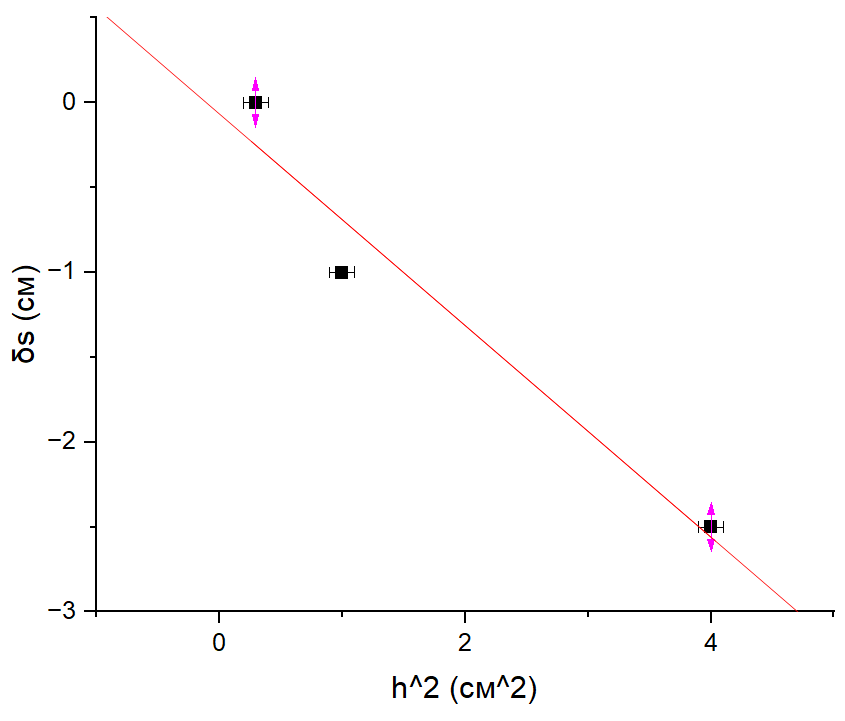
\includegraphics[width=0.65\textwidth]{4.1.1_10.png}\\
\textbf{Рис. 10.} График зависимости отклонения от начального положения от квадрата диаметра диафрагмы $\delta s (h^2)$ \\
\end{center}

\hfill \break Обратимся к формулам (17) и (18):

$$
s(h) = - \frac {n^2} {2R(n - 1)} h^2 + \frac {R} {n - 1},
$$

\hfill \break откуда $k = - \frac {n^2} {2R(n - 1)}$ и $b = \frac {R} {n - 1}$, $\Rightarrow k = - \frac {n^2} {2b(n-1)^2}$; отсюда можно найти \textbf{показатель преломления стекла линзы}:

$$
n = \frac {4kb + \sqrt{-8kb}} {4kb + 2} \approx 1.53 \pm 0.03,
$$

\hfill \break где $k$ и $b$ $-$ коэффициенты прямой на графике, которую можно представить в виде $y = kx + b$.

\subsubsection*{II. Хроматическая аберрация}
\hfill \break Используя зрительную трубу и три светофильтра (красный, желтый и синий), определим по нониусной шкале положения плосковыпуклой линзы, соответствующие резкому изображению предмета. 

\hfill \break Фокусное расстояние линзы №3, измеренное с желтым светофильтром, $-$ $f_{D} = (70.5 \pm 0.1)$ мм, с голубым $-$ $f_{F} = (69.2 \pm 0.1)$ мм, с красным $-$ $f_{C} = (70.7 \pm 0.1)$ мм.

\hfill \break Рассчитаем \textbf{хроматическую аберрацию} по формуле (19) $\delta f_{\text{хр}} = f_{F} - f_{C} = -1.5$ мм и \textbf{число Аббе} по формуле (21):

$$
\nu = - \frac {f_{D}} {\delta f_{\text{хр}}} = 47.
$$

\section{Вывод}
\hfill \break В данной лабораторной работе были изучены центрированные оптические системы. Разными способами были определены фокусные расстояния собирающих и рассеивающих линз, исследованы явления сферической и хроматической аберраций оптических систем.

\end{document}
